%%%%%%%%%%%%%%%%%%%%%%%%%%%%%%%%%%%%%%%%%%%%%%%%%%%%%%%%%%%%%%%%%%%%%%%%%%%%%%%%%%
\begin{frame}[fragile]\frametitle{}
\begin{center}
{\Large Introduction}
\end{center}
\end{frame}



%%%%%%%%%%%%%%%%%%%%%%%%%%%%%%%%%%%%%%%%%%%%%%%%%%%%%%%%%%%
\begin{frame}[fragile]\frametitle{Intuition}

\begin{itemize}
\item Graph: Nodes connected by Edges
\item Knowledge Graph: Entities connected by Relations.
\end{itemize}
	  
\end{frame}




%%%%%%%%%%%%%%%%%%%%%%%%%%%%%%%%%%%%%%%%%%%%%%%%%%%%%%%%%%%%%%%%%%%%%%%%%%%%%%%%%%
\begin{frame}\frametitle{A Graph is}
{\emph \ldots a set of discrete objects, each of which has some set of relationships with the other objects}

Euler: Can we take a walk to all 4 islands, without crossing any of the bridge twice?

Abstraction (Does size of islands matter?):

\begin{center}
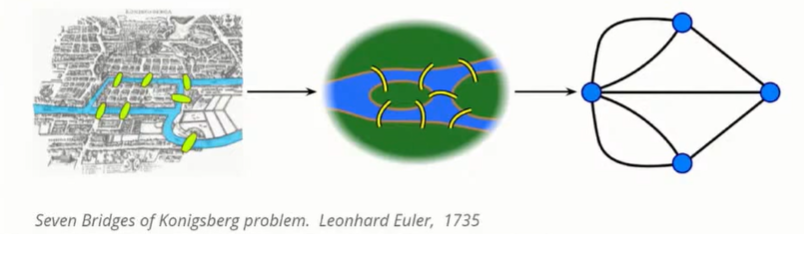
\includegraphics[width=\linewidth,keepaspectratio]{neo4j4}
\end{center}	  

Solution: No way!! What's the rule?

{\tiny (Ref: Introduction to Neo4j - a hands-on crash course - neo4j)}
\end{frame}


%%%%%%%%%%%%%%%%%%%%%%%%%%%%%%%%%%%%%%%%%%%%%%%%%%%%%%%%%%%
\begin{frame}[fragile]\frametitle{ Graph-structured Data Are Ubiquitous }

\begin{center}
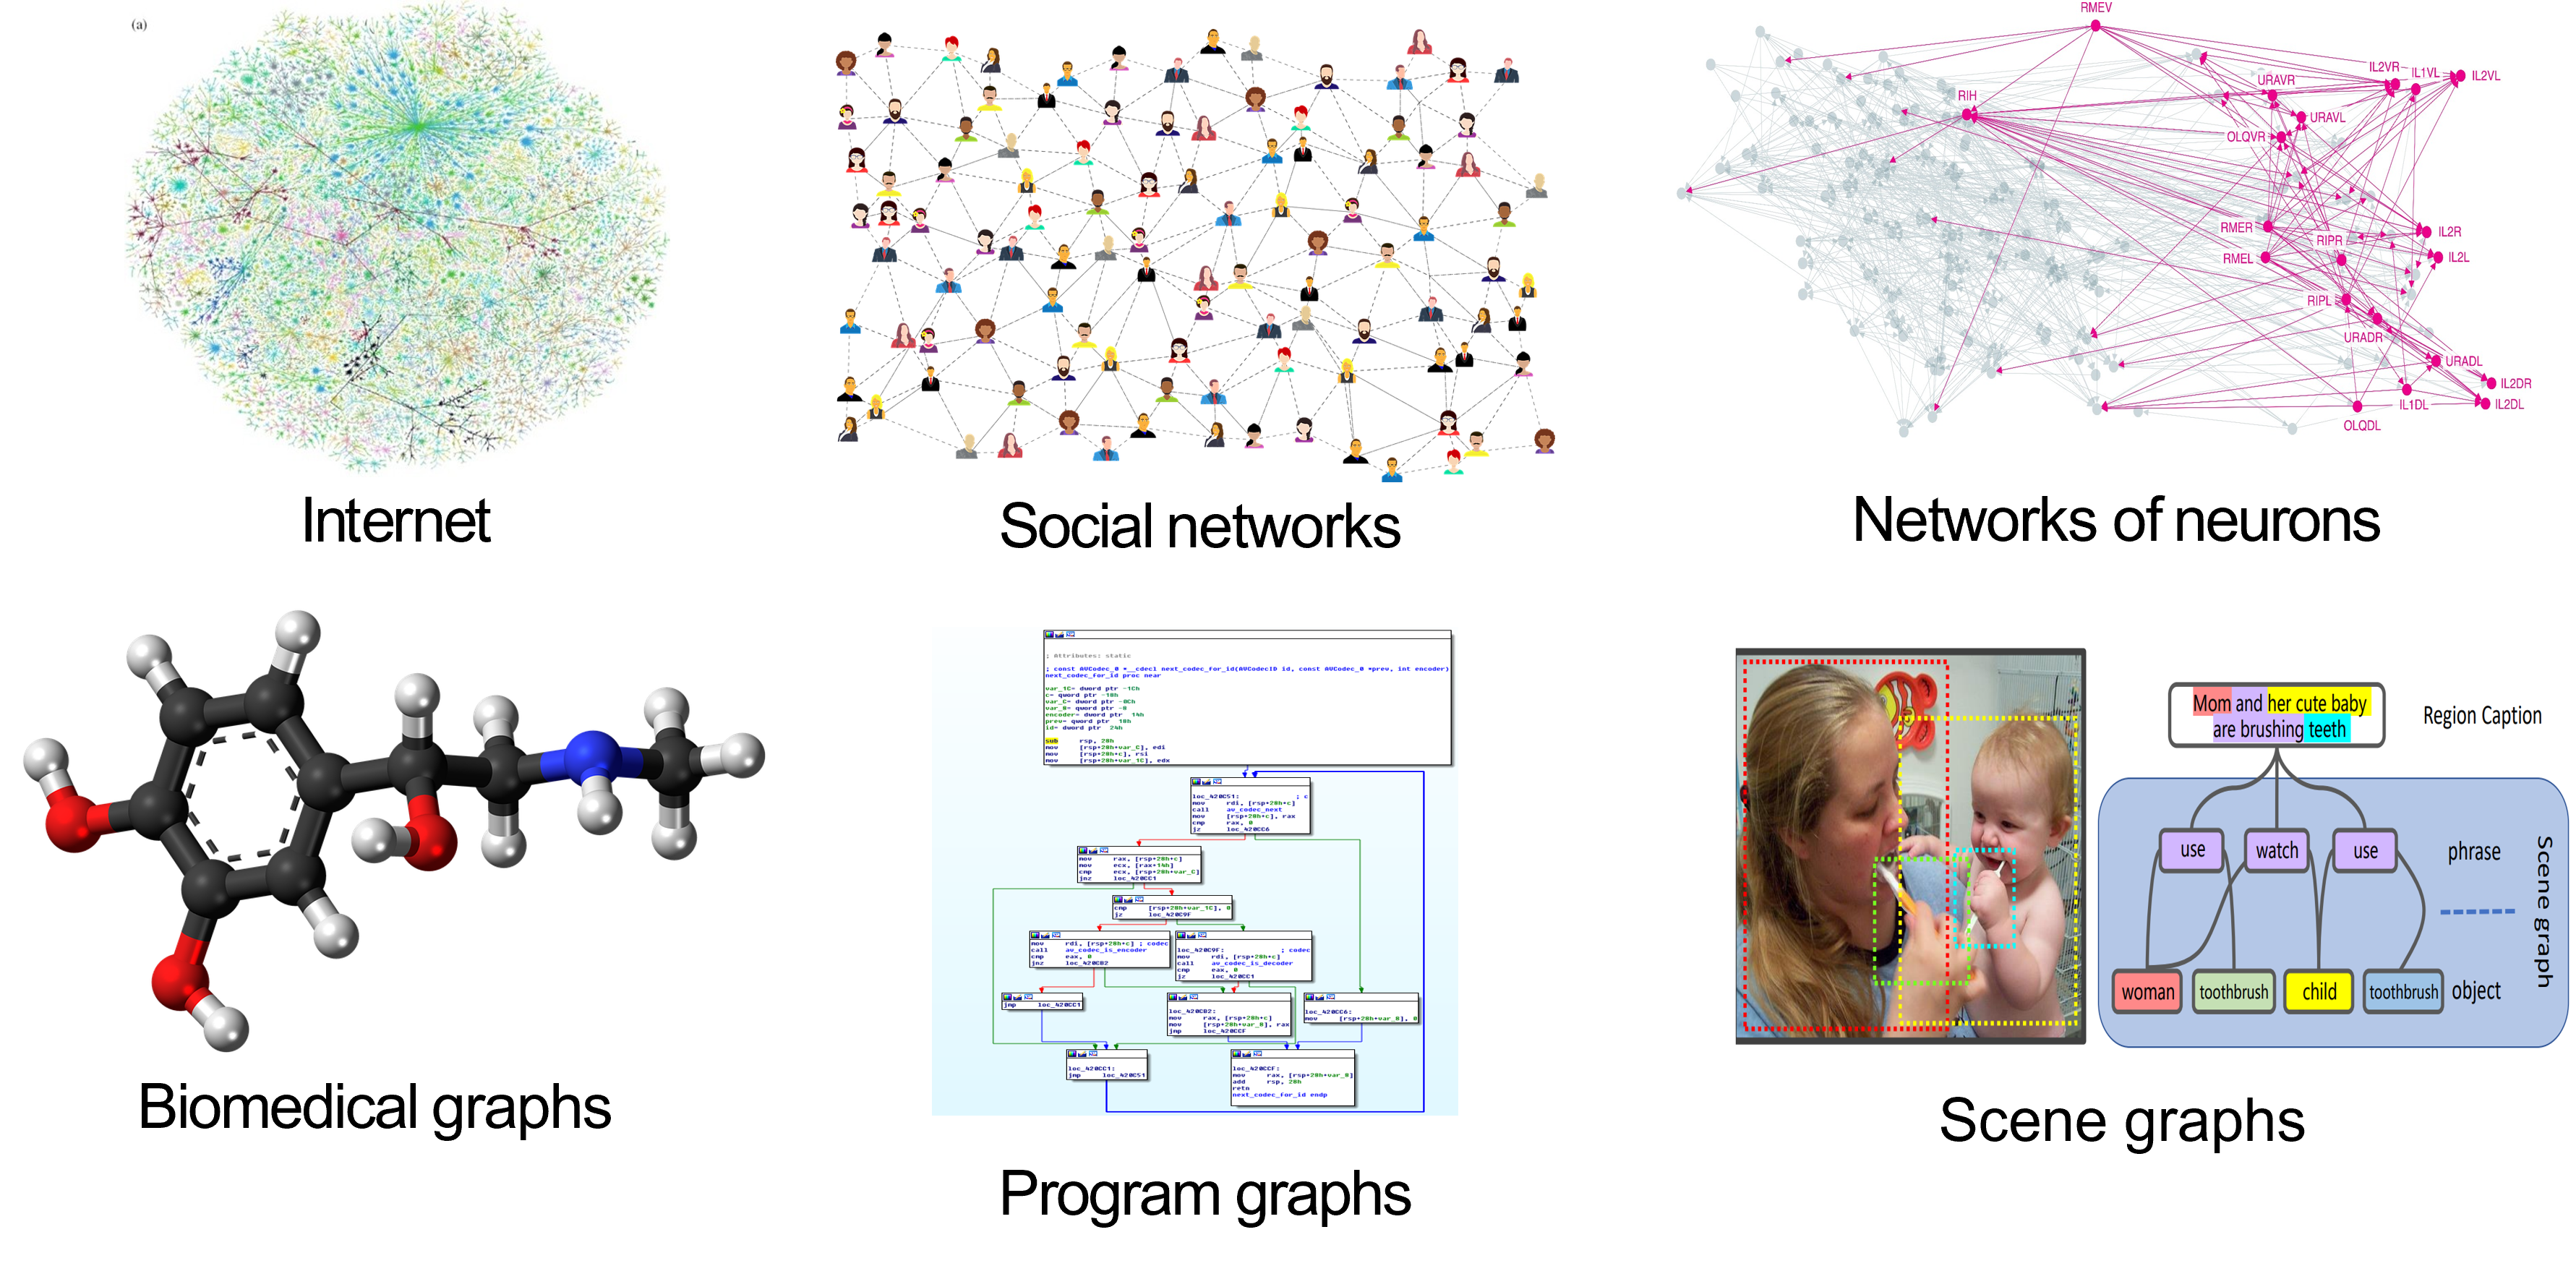
\includegraphics[width=\linewidth,keepaspectratio]{gnn1}
\end{center}	  

\end{frame}



%%%%%%%%%%%%%%%%%%%%%%%%%%%%%%%%%%%%%%%%%%%%%%%%%%%%%%%%%%%
\begin{frame}[fragile]\frametitle{Graphs: A Universal Language }

\begin{center}
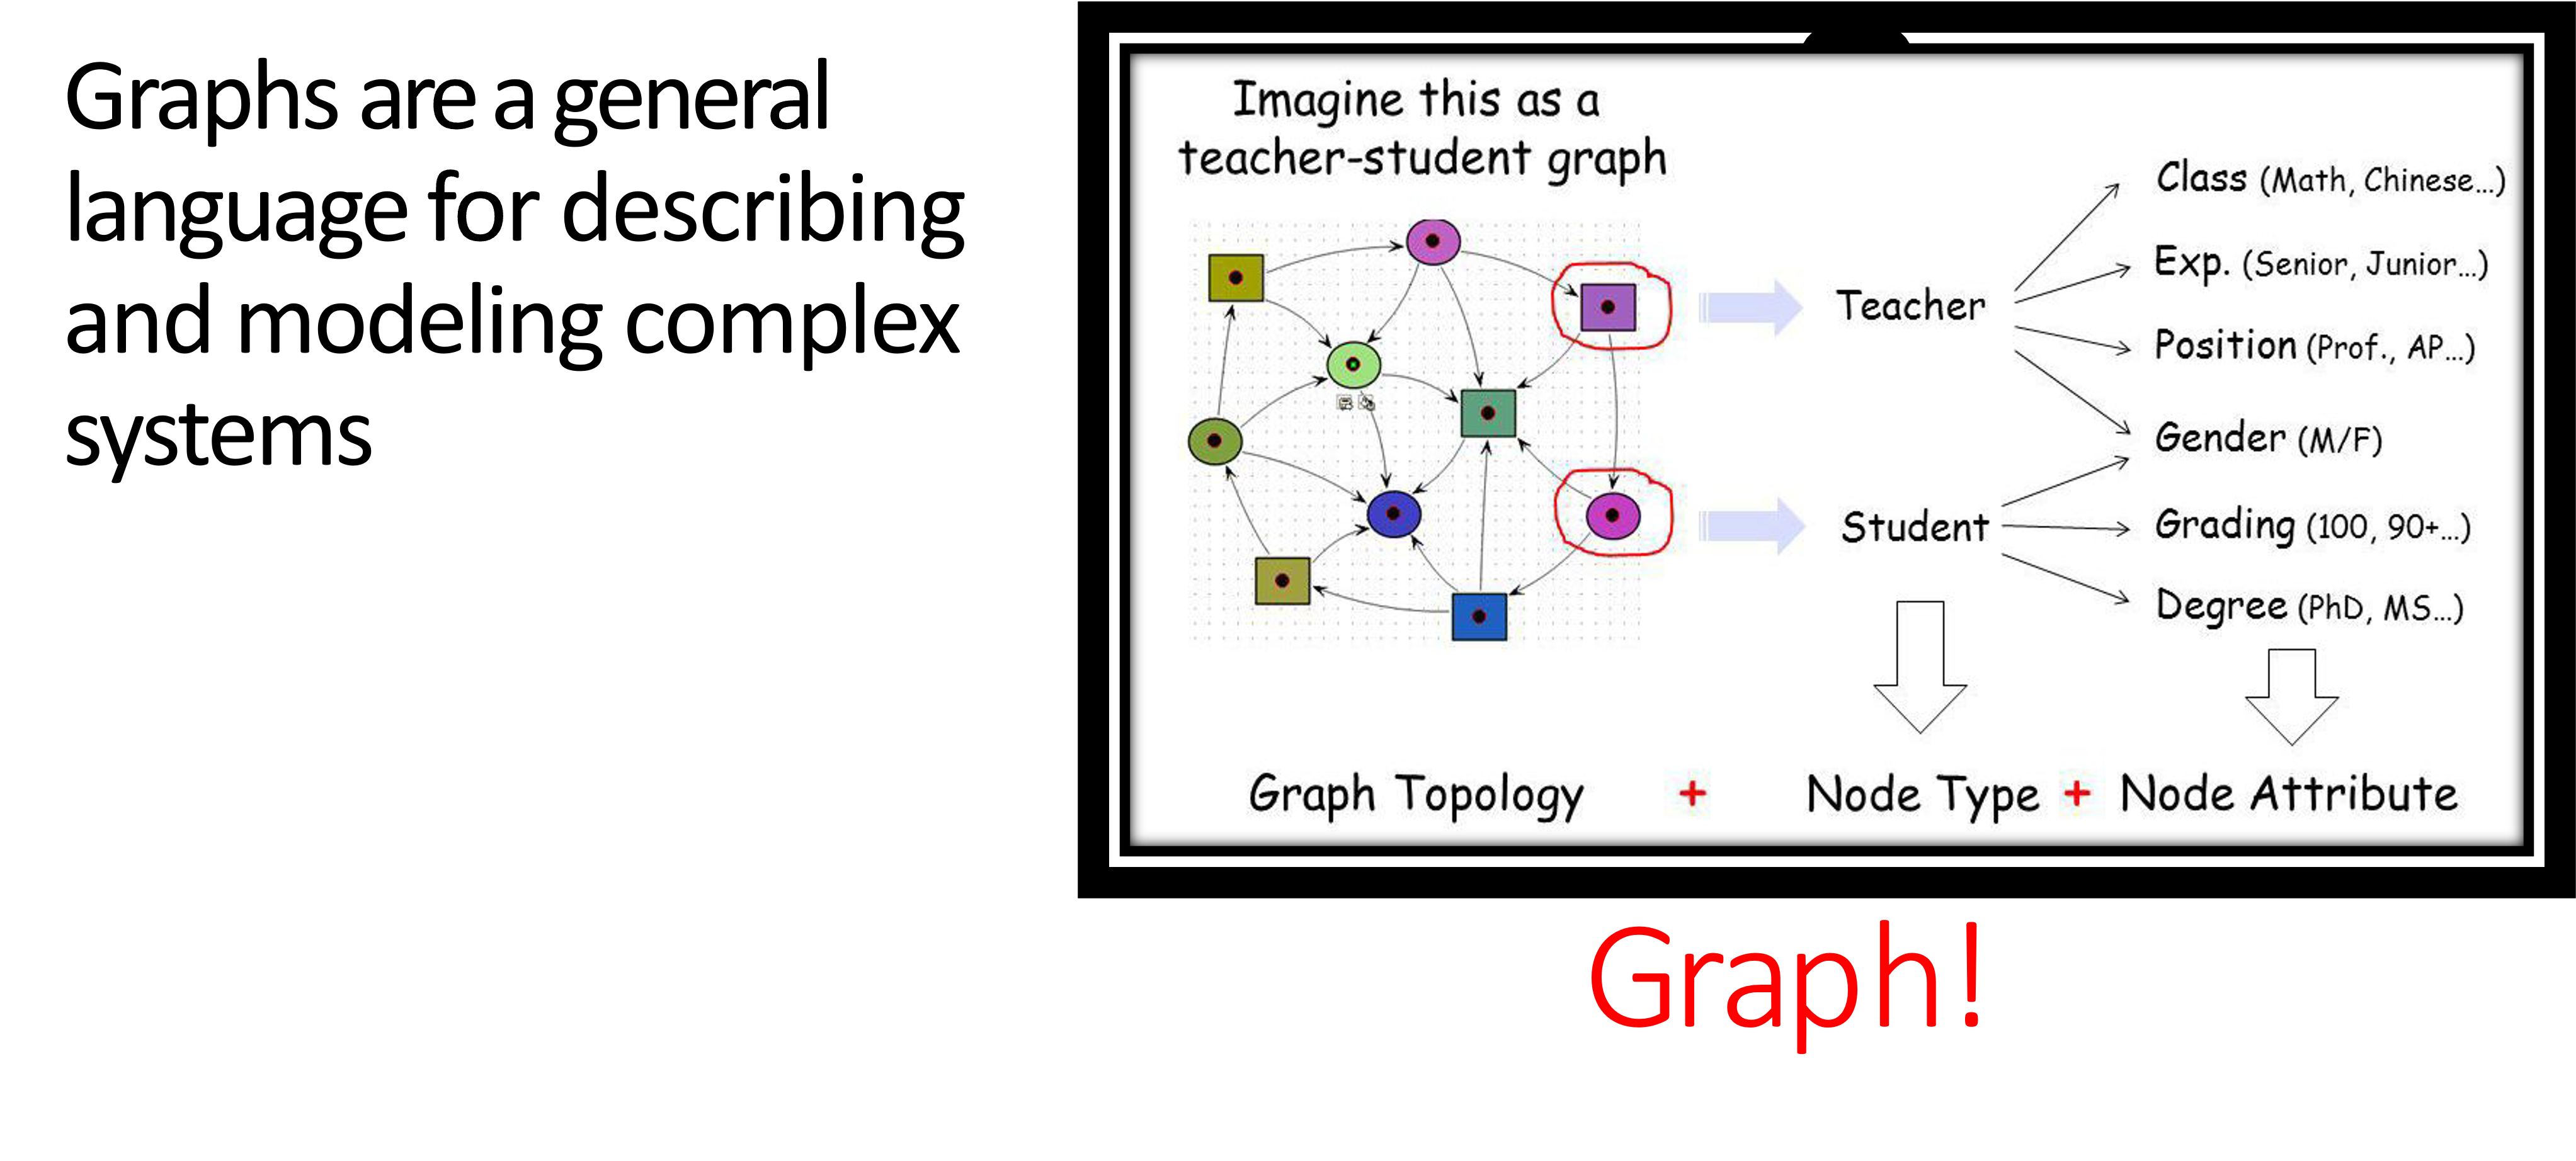
\includegraphics[width=\linewidth,keepaspectratio]{gnn4}
\end{center}	  

\end{frame}


%%%%%%%%%%%%%%%%%%%%%%%%%%%%%%%%%%%%%%%%%%%%%%%%%%%%%%%%%%%
\begin{frame}[fragile]\frametitle{Data as Graphs - Explicit }

\begin{center}
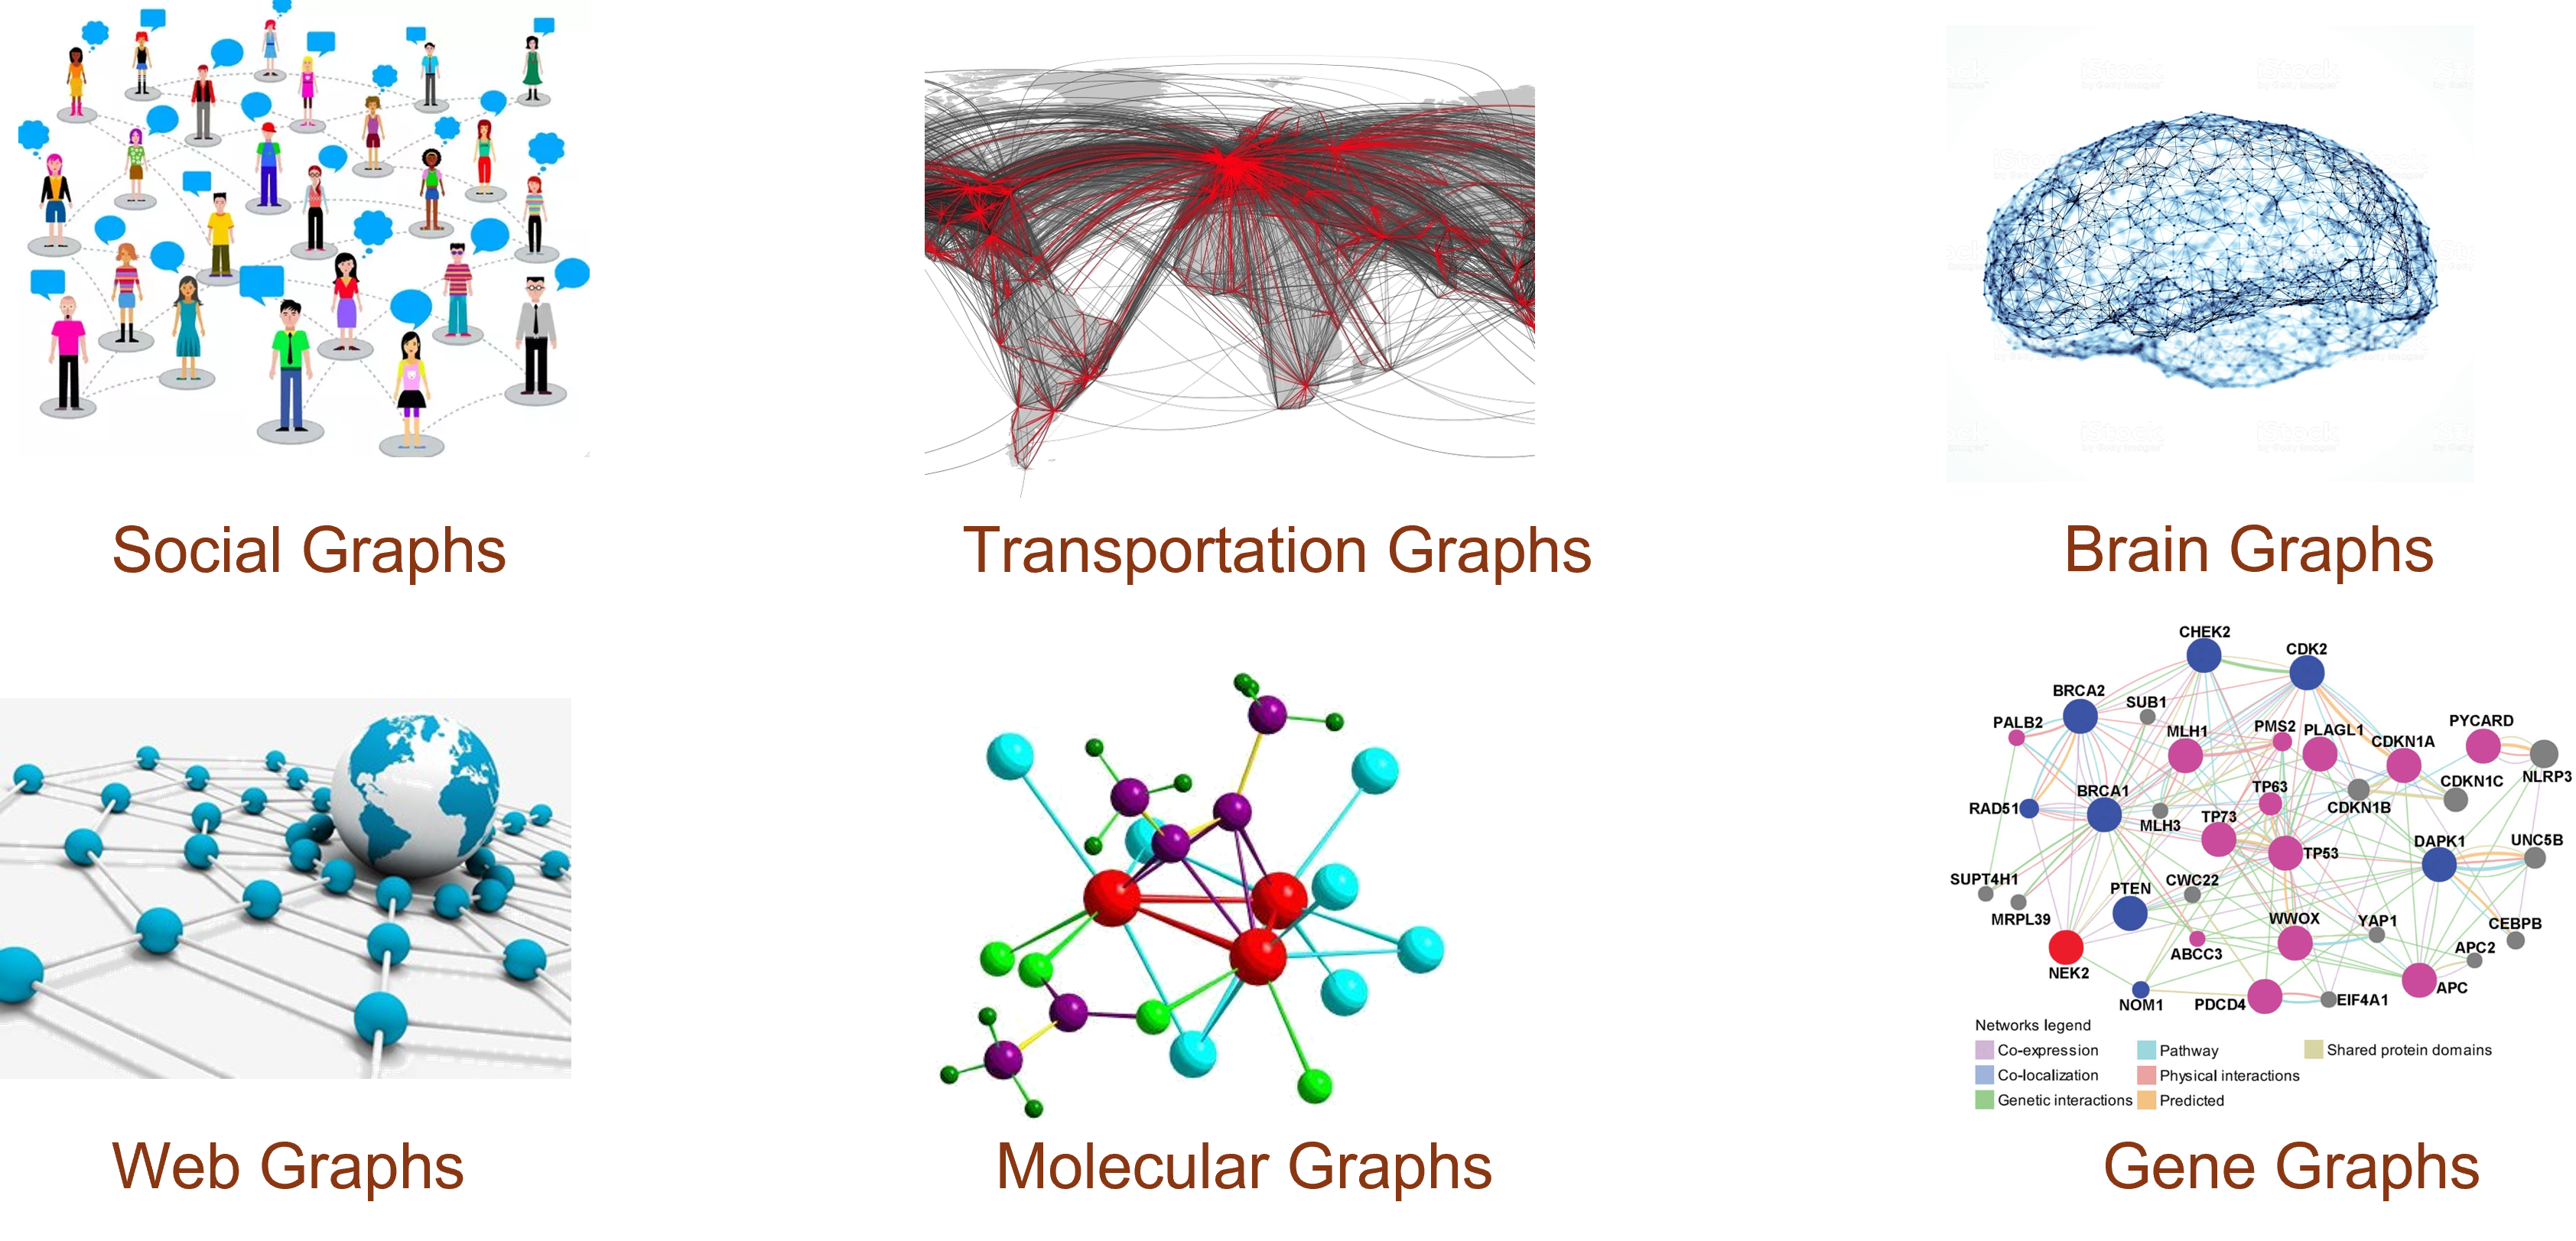
\includegraphics[width=\linewidth,keepaspectratio]{gnn5}
\end{center}	  

\end{frame}

%%%%%%%%%%%%%%%%%%%%%%%%%%%%%%%%%%%%%%%%%%%%%%%%%%%%%%%%%%%
\begin{frame}[fragile]\frametitle{Data as Graphs - Implicit }

\begin{center}
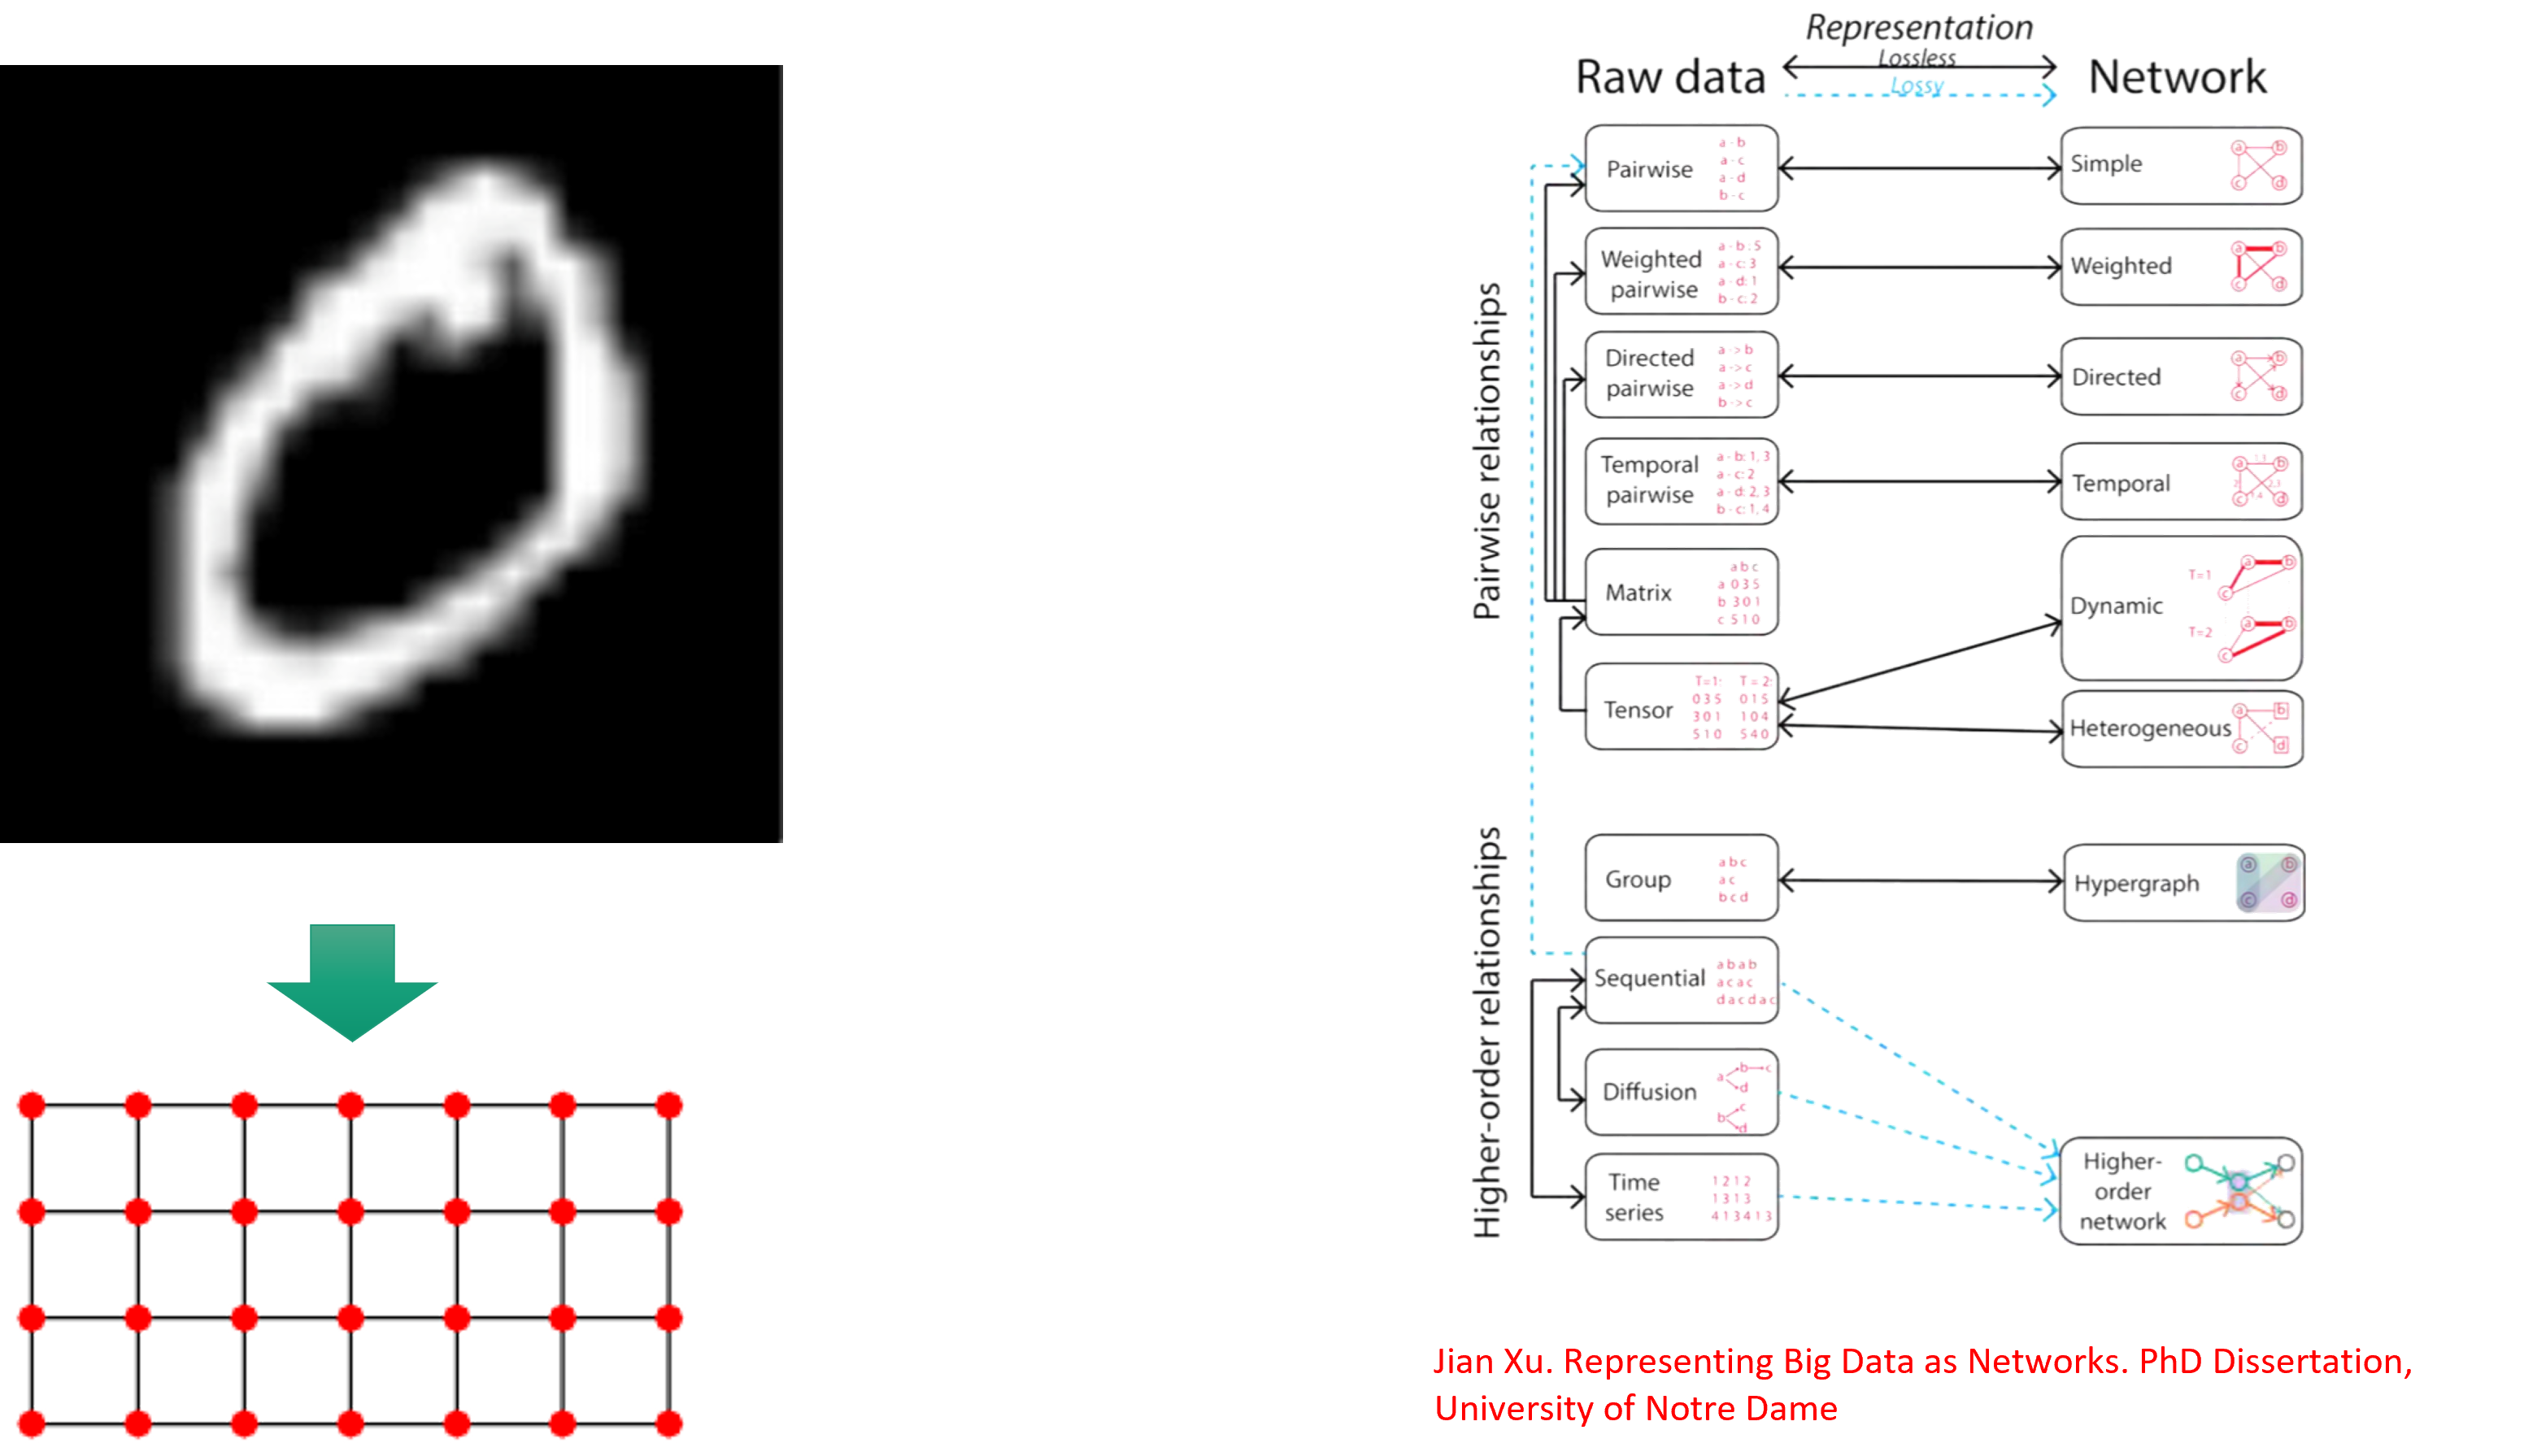
\includegraphics[width=\linewidth,keepaspectratio]{gnn6}
\end{center}	  

\end{frame}


%%%%%%%%%%%%%%%%%%%%%%%%%%%%%%%%%%%%%%%%%%%%%%%%%%%%%%%%%%%%%%%%%%%%%%%%%%%%%%%%%%
\begin{frame}\frametitle{ Graph Applications }

Across an organization, every department can benefit from graphs to answer questions 
like who or what is important, what should I do next, and what’s unusual about this?

\begin{center}
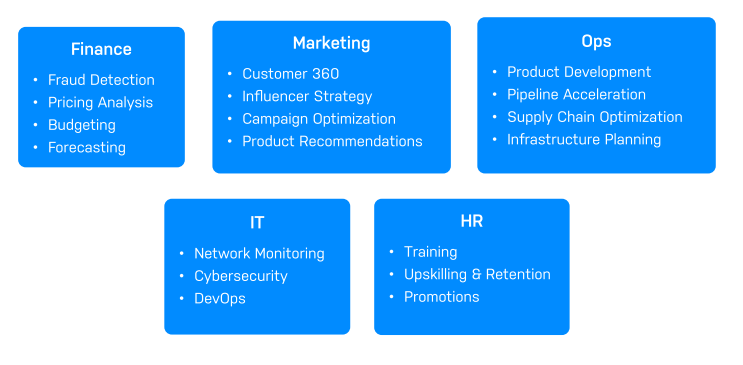
\includegraphics[width=\linewidth,keepaspectratio]{neo4j103}
\end{center}	  


{\tiny (Ref: 5 Graph Data Science Basics Everyone Should Know - neo4j)}
\end{frame}

%%%%%%%%%%%%%%%%%%%%%%%%%%%%%%%%%%%%%%%%%%%%%%%%%%%%%%%%%%%
\begin{frame}[fragile]\frametitle{A Knowledge Graph is}
 
\begin{center}
{\em \ldots an interconnected dataset enriched with meaning so we can reason about the underlying data and use it confidently for complex decision making}
\end{center}

	  - A neo4j definition
		
\end{frame}


%%%%%%%%%%%%%%%%%%%%%%%%%%%%%%%%%%%%%%%%%%%%%%%%%%%%%%%%%%%
\begin{frame}[fragile]\frametitle{A progression}
 
 of more enrichment \ldots
 
			\begin{center}
			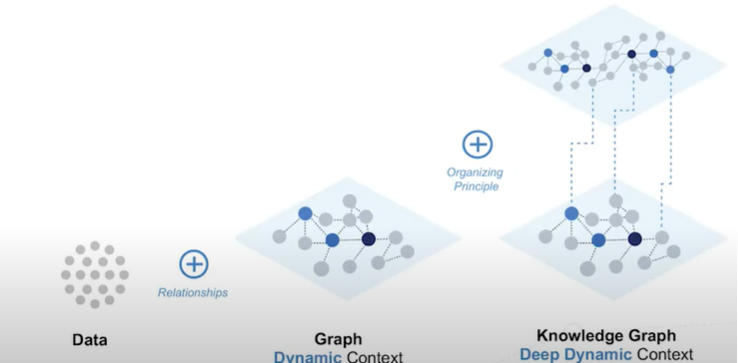
\includegraphics[width=\linewidth,keepaspectratio]{kg5}
			\end{center}	
			
			{\tiny (Ref: A Universe of Knowledge Graphs - neo4j)}
		
\end{frame}

%%%%%%%%%%%%%%%%%%%%%%%%%%%%%%%%%%%%%%%%%%%%%%%%%%%%%%%%%%%
\begin{frame}[fragile]\frametitle{Data}
 
 Variety of type/organization of data
 
			\begin{center}
			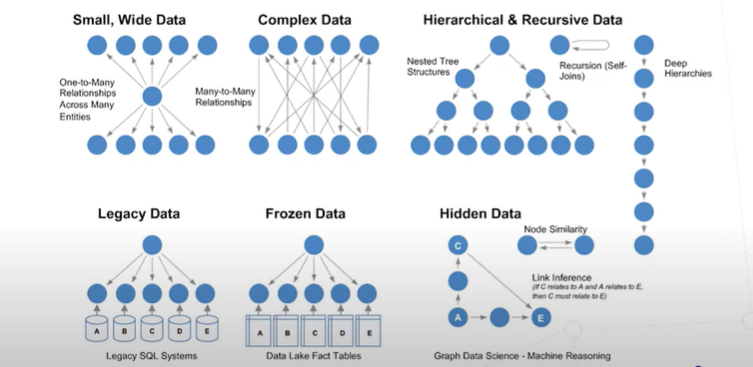
\includegraphics[width=\linewidth,keepaspectratio]{kg6}
			\end{center}	
			
			{\tiny (Ref: A Universe of Knowledge Graphs - neo4j)}
		
		
		``No more a Big Data but need Small and Wide data'' for more context in Machine Learning.
		
\end{frame}

%%%%%%%%%%%%%%%%%%%%%%%%%%%%%%%%%%%%%%%%%%%%%%%%%%%%%%%%%%%
\begin{frame}[fragile]\frametitle{Graphs}
 
 add Relationships to Data \ldots
 
 
			\begin{center}
			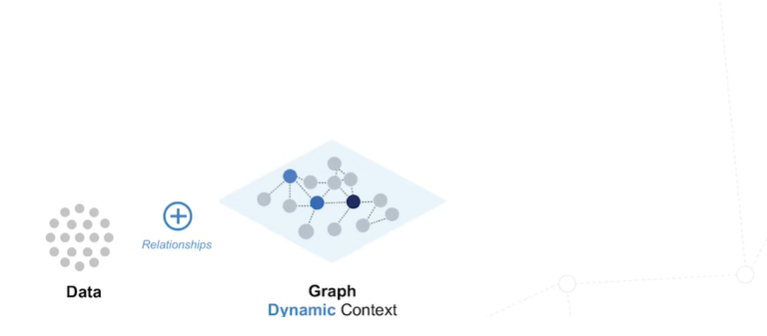
\includegraphics[width=\linewidth,keepaspectratio]{kg7}
			\end{center}	
			
			{\tiny (Ref: A Universe of Knowledge Graphs - neo4j)}
		
		
\end{frame}

%%%%%%%%%%%%%%%%%%%%%%%%%%%%%%%%%%%%%%%%%%%%%%%%%%%%%%%%%%%
\begin{frame}[fragile]\frametitle{Knowledge Graphs}
 
 add Organizing principles to Graphs \ldots
 
 
			\begin{center}
			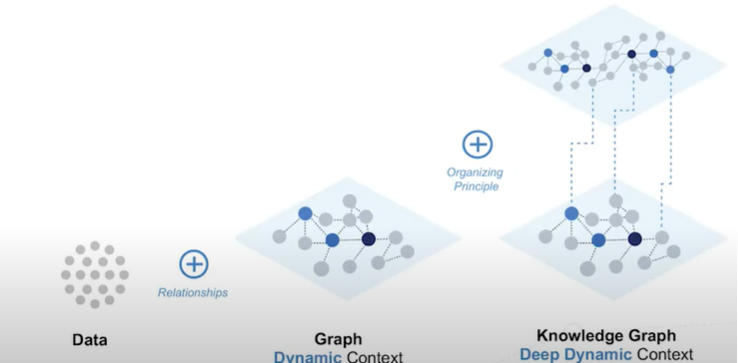
\includegraphics[width=\linewidth,keepaspectratio]{kg5}
			\end{center}	
			
			{\tiny (Ref: A Universe of Knowledge Graphs - neo4j)}
		
		e.g. external knowledge, ontologies injection. or 'Semantics'
		
\end{frame}


%%%%%%%%%%%%%%%%%%%%%%%%%%%%%%%%%%%%%%%%%%%%%%%%%%%%%%%%%%%
\begin{frame}[fragile]\frametitle{Semantics}
 
Semantics = Context = Domain Knowledge. 
 
			\begin{center}
			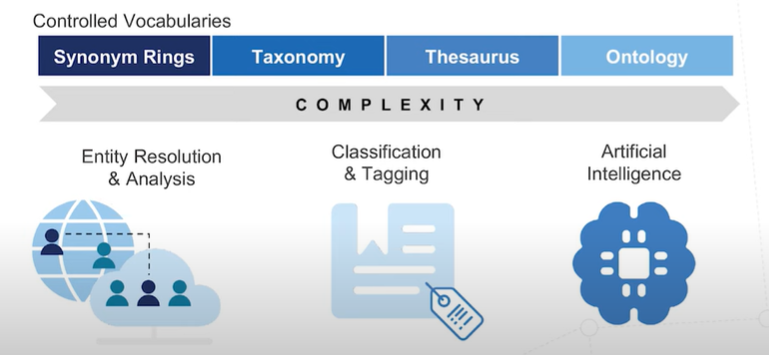
\includegraphics[width=\linewidth,keepaspectratio]{kg8}
			\end{center}	
			
			{\tiny (Ref: A Universe of Knowledge Graphs - neo4j)}
		
	
\end{frame}

%%%%%%%%%%%%%%%%%%%%%%%%%%%%%%%%%%%%%%%%%%%%%%%%%%%%%%%%%%%%%%%%%%%%%%%%%%%%%%%%%%
\begin{frame}\frametitle{So, a Knowledge Graph is}


\begin{columns}
    \begin{column}[T]{0.6\linewidth}

		Knowledge in Graph form.

			\begin{center}
			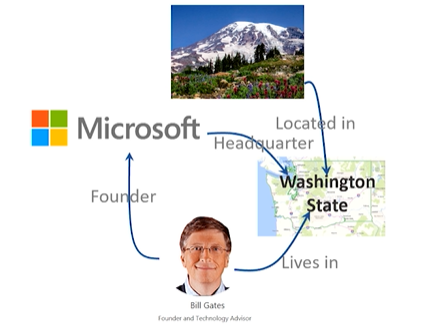
\includegraphics[width=\linewidth,keepaspectratio]{kg1}
			\end{center}	
    \end{column}
    \begin{column}[T]{0.4\linewidth}
			Embedded knowledge is:
			\begin{itemize}
			\item Microsoft is headquartered in Washington State.
			\item Bill Gates is a (co)Founder of Microsoft
			\item etc.
			\item Entities: Microsoft, Washington State, etc
			\item Relationships: founder, head, etc.
			\end{itemize}
    \end{column}
  \end{columns}
	

  

{\tiny (Ref: DAT278x - From Graph and Knowledge Graph - EdX course)}
\end{frame}


%%%%%%%%%%%%%%%%%%%%%%%%%%%%%%%%%%%%%%%%%%%%%%%%%%%%%%%%%%%%%%%%%%%%%%%%%%%%%%%%%%
\begin{frame}\frametitle{A Knowledge Graph is}

\begin{center}
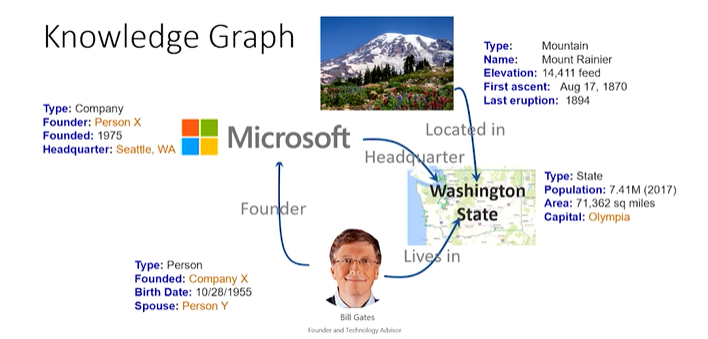
\includegraphics[width=\linewidth,keepaspectratio]{kg2}
\end{center}	

\begin{itemize}
\item Entities can be locations, companies, persons, etc. Nouns
\item Relationships can actions, has-a, etc. Verbs.
\end{itemize}


{\tiny (Ref: DAT278x - From Graph and Knowledge Graph - EdX course)}
\end{frame}

%%%%%%%%%%%%%%%%%%%%%%%%%%%%%%%%%%%%%%%%%%%%%%%%%%%%%%%%%%%%%%%%%%%%%%%%%%%%%%%%%%
\begin{frame}\frametitle{Knowledge Graph Datasets}

\begin{center}
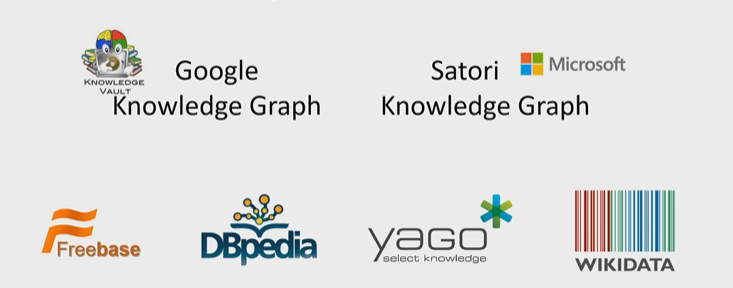
\includegraphics[width=\linewidth,keepaspectratio]{kg3}
\end{center}	

\begin{itemize}
\item Google, Microsoft KGs are private and used for search, question answering
\item DBPedia, Wikidata KGs are public
\end{itemize}

{\tiny (Ref: DAT278x - From Graph and Knowledge Graph - EdX course)}
\end{frame}

%%%%%%%%%%%%%%%%%%%%%%%%%%%%%%%%%%%%%%%%%%%%%%%%%%%%%%%%%%%%%%%%%%%%%%%%%%%%%%%%%%
\begin{frame}\frametitle{Domain specific Knowledge Graphs}

\begin{center}
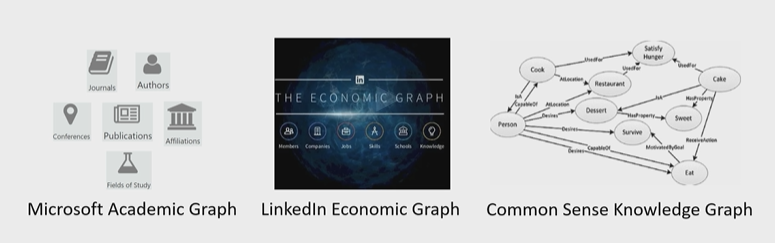
\includegraphics[width=\linewidth,keepaspectratio]{kg4}
\end{center}	


\begin{itemize}
\item Microsoft Academic Graph has 170 million papers and more than 200 million authors
\item LinkedIn Economic Graph has 500 million members and 20 million companies.
\end{itemize}

{\tiny (Ref: DAT278x - From Graph and Knowledge Graph - EdX course)}
\end{frame}


%%%%%%%%%%%%%%%%%%%%%%%%%%%%%%%%%%%%%%%%%%%%%%%%%%%%%%%%%%%%%%%%%%%%%%%%%%%%%%%%%%
\begin{frame}\frametitle{Why knowledge graph is important?}

\begin{itemize}
\item Help organize information
\item Tackle information overload
\item Intuitive explanation, visualization
\item Supports easy querying and business decisions.
\item Key component in many AI applications like Chatbot
\end{itemize}

{\tiny (Ref: DAT278x - From Graph and Knowledge Graph - EdX course)}
\end{frame}

%%%%%%%%%%%%%%%%%%%%%%%%%%%%%%%%%%%%%%%%%%%%%%%%%%%%%%%%%%%
\begin{frame}[fragile]\frametitle{Applications}
 
 
			\begin{center}
			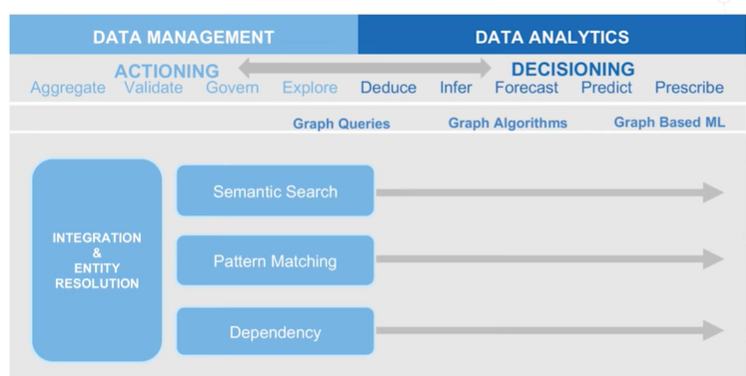
\includegraphics[width=\linewidth,keepaspectratio]{kg9}
			\end{center}	
			
			{\tiny (Ref: A Universe of Knowledge Graphs - neo4j)}
		
	
\end{frame}

%%%%%%%%%%%%%%%%%%%%%%%%%%%%%%%%%%%%%%%%%%%%%%%%%%%%%%%%%%%
\begin{frame}[fragile]\frametitle{Applications}
 
 Bridge data Silos
 
			\begin{center}
			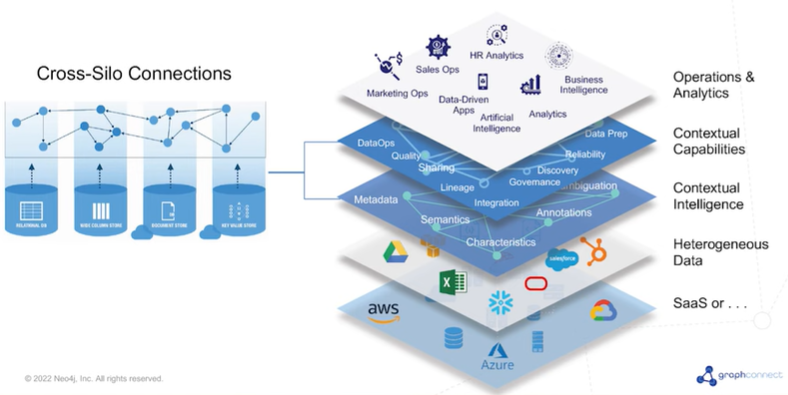
\includegraphics[width=\linewidth,keepaspectratio]{kg10}
			\end{center}	
			
			{\tiny (Ref: A Universe of Knowledge Graphs - neo4j)}
		
	
\end{frame}



%%%%%%%%%%%%%%%%%%%%%%%%%%%%%%%%%%%%%%%%%%%%%%%%%%%%%%%%%%%%%%%%%%%%%%%%%%%%%%%%%%
\begin{frame}\frametitle{Applications}

\begin{itemize}
\item Entity recommendation (Google right hand box): Searching via associated keywords
\item Semantic Search and recommendations using click logs
\item Personal Assistant like Alexa, Siri, using information associated with you.
\end{itemize}

{\tiny (Ref: DAT278x - From Graph and Knowledge Graph - EdX course)}
\end{frame}


%%%%%%%%%%%%%%%%%%%%%%%%%%%%%%%%%%%%%%%%%%%%%%%%%%%%%%%%%%%
\begin{frame}[fragile]\frametitle{Semantic Search}
 
 
			\begin{center}
			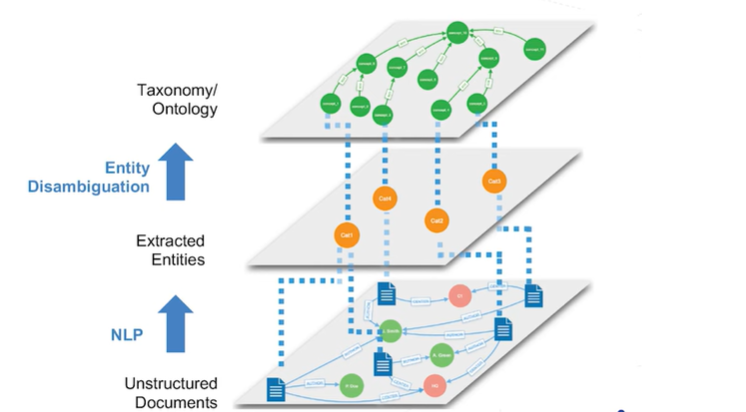
\includegraphics[width=\linewidth,keepaspectratio]{kg11}
			\end{center}	
			
			{\tiny (Ref: A Universe of Knowledge Graphs - neo4j)}
		
	
\end{frame}

%%%%%%%%%%%%%%%%%%%%%%%%%%%%%%%%%%%%%%%%%%%%%%%%%%%%%%%%%%%
\begin{frame}[fragile]\frametitle{Implicit Relationships}
 
	Candidate to Job matching via skills
 
			\begin{center}
			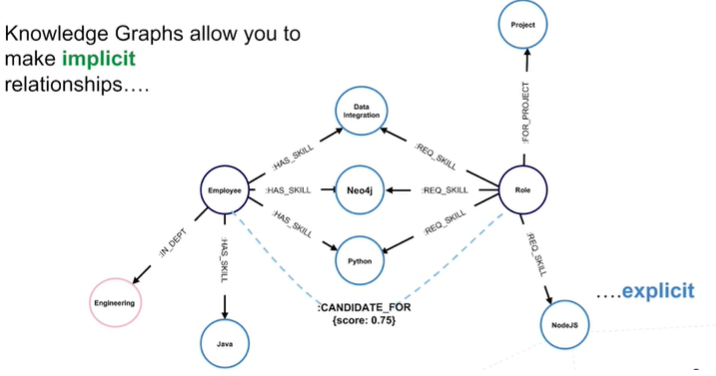
\includegraphics[width=\linewidth,keepaspectratio]{kg12}
			\end{center}	
			
			{\tiny (Ref: A Universe of Knowledge Graphs - neo4j)}
		
	
\end{frame}

%%%%%%%%%%%%%%%%%%%%%%%%%%%%%%%%%%%%%%%%%%%%%%%%%%%%%%%%%%%
\begin{frame}[fragile]\frametitle{Hidden Insights}
 
 
			\begin{center}
			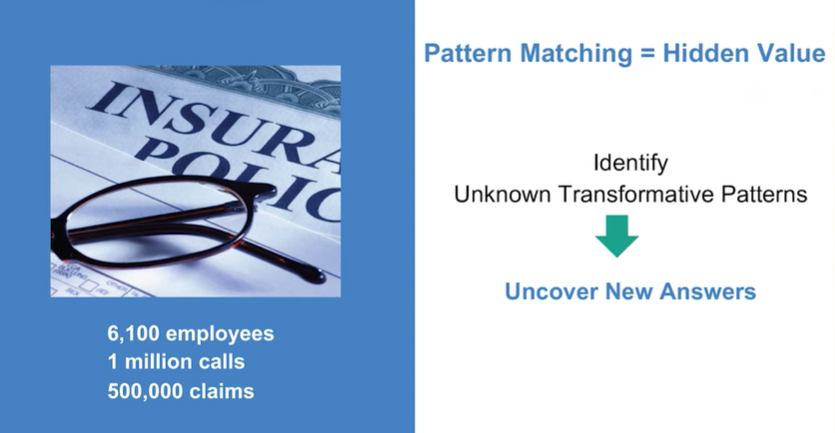
\includegraphics[width=\linewidth,keepaspectratio]{kg13}
			\end{center}	
			
			{\tiny (Ref: A Universe of Knowledge Graphs - neo4j)}
		
	
\end{frame}

%%%%%%%%%%%%%%%%%%%%%%%%%%%%%%%%%%%%%%%%%%%%%%%%%%%%%%%%%%%
\begin{frame}[fragile]\frametitle{Usages}
 
 
			\begin{center}
			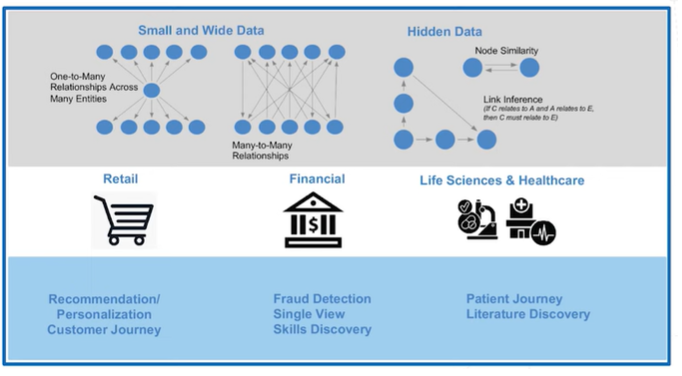
\includegraphics[width=\linewidth,keepaspectratio]{kg14}
			\end{center}	
			
			{\tiny (Ref: A Universe of Knowledge Graphs - neo4j)}
		
	
\end{frame}

%%%%%%%%%%%%%%%%%%%%%%%%%%%%%%%%%%%%%%%%%%%%%%%%%%%%%%%%%%%
\begin{frame}[fragile]\frametitle{Criticality}
 
 
			\begin{center}
			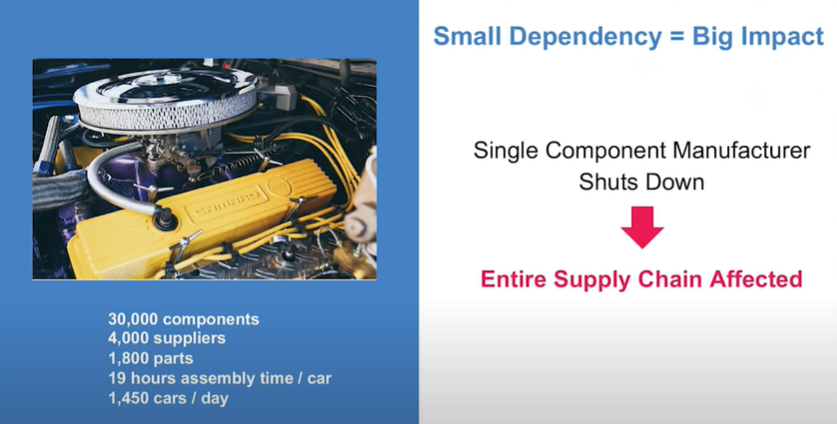
\includegraphics[width=\linewidth,keepaspectratio]{kg15}
			\end{center}	
			
			{\tiny (Ref: A Universe of Knowledge Graphs - neo4j)}
		
	
\end{frame}



%%%%%%%%%%%%%%%%%%%%%%%%%%%%%%%%%%%%%%%%%%%%%%%%%%%%%%%%%%%%%%%%%%%%%%%%%%%%%%%%%%
\begin{frame}[fragile]\frametitle{}
\begin{center}
{\Large Implementation}
\end{center}
\end{frame}



%%%%%%%%%%%%%%%%%%%%%%%%%%%%%%%%%%%%%%%%%%%%%%%%%%%%%%%%%%%
\begin{frame}[fragile]\frametitle{Problem Statement}

\begin{itemize}
\item Traditional job recommendation systems are based on simple keyword and/or semantic similarity that are usually not well suited to providing good job recommendations since they don’t take into account the interlinks between entities. 
\item It is of utmost importance to have field-relevant skills listed on your resume and to uncover which industry skills are becoming more pertinent.
\item For instance, I might have extensive skills in Python programming, but the job description of interest requires knowledge in Django framework, which is essentially based on Python; a simple keyword search will miss that connection.
\item Build a job recommendation and skill discovery script that will take unstructured text as input, and will then output job recommendations and skill suggestions based on entities such as skills, years of experience, diploma, and major
\end{itemize}
	  
			\begin{center}
			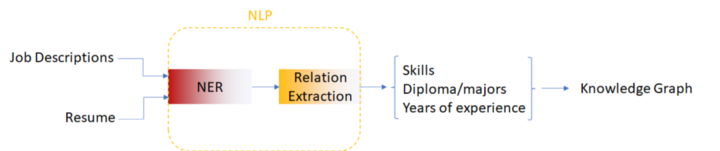
\includegraphics[width=0.8\linewidth,keepaspectratio]{kg16}
			\end{center}	
			
			{\tiny (Ref: Building a Knowledge Graph for Job Search using BERT Transformer - Walid Amamou)}		
\end{frame}



%%%%%%%%%%%%%%%%%%%%%%%%%%%%%%%%%%%%%%%%%%%%%%%%%%%%%%%%%%%
\begin{frame}[fragile]\frametitle{Choice}

\begin{itemize}
\item PoC: possible with NER and python library networkX, but its limited as the whole graphs stays in memory. Cant scale.
\item Need graph database, say, Neo4j.
\item Can store large amounts of data (nodes, edges) and has intuitive query language called, Cypher.
\end{itemize}
	  
\end{frame}

%%%%%%%%%%%%%%%%%%%%%%%%%%%%%%%%%%%%%%%%%%%%%%%%%%%%%%%%%%%
\begin{frame}[fragile]\frametitle{Steps}

\begin{itemize}
\item Generate training data. Publicly available in Kaggle (https://www.kaggle.com/airiddha/trainrev1)
\item Load our fine-tuned transformer NER and spacy relation extraction model
\item Create a Neo4j Sandbox and add our entities and relations
\item Query our graph to find the highest job match to a target resume, find the three most popular skills and highest skills co-occurrence
\end{itemize}
	  
\end{frame}


%%%%%%%%%%%%%%%%%%%%%%%%%%%%%%%%%%%%%%%%%%%%%%%%%%%%%%%%%%%
\begin{frame}[fragile]\frametitle{Data Extraction}

Load the jobs dataset:


\begin{lstlisting}
import pandas as pd
def get_all_documents():
	df = pd.read_csv("/content/drive/MyDrive/job_DB1_1_29.csv",sep='"',header=None)
	documents = []
	for index,row in df.iterrows():
			documents.append(str(row[0]))
			return documents
	documents = get_all_documents()
	documents = documents[:]
\end{lstlisting}
	  
\end{frame}

%%%%%%%%%%%%%%%%%%%%%%%%%%%%%%%%%%%%%%%%%%%%%%%%%%%%%%%%%%%
\begin{frame}[fragile]\frametitle{Named Entity and Relation Extraction}

Install and Load:


\begin{lstlisting}
!pip install -U pip setuptools wheel
!python -m spacy project clone tutorials/rel_component
!pip install -U spacy-nightly --pre
!!pip install -U spacy transformers
import spacy
#restart the runtime after installation of deps
nlp = spacy.load("[PATH_TO_THE_MODEL]/model-best")
\end{lstlisting}
	  
\end{frame}


%%%%%%%%%%%%%%%%%%%%%%%%%%%%%%%%%%%%%%%%%%%%%%%%%%%%%%%%%%%
\begin{frame}[fragile]\frametitle{Prepare Training Data}

Extract entities from the jobs dataset:

\begin{lstlisting}
import hashlib
def extract_ents(documents,nlp):
  docs = list()
  for doc in nlp.pipe(documents, disable=["tagger", "parser"]):
      dictionary=dict.fromkeys(["text", "annotations"])
      dictionary["text"]= str(doc)
      dictionary['text_sha256'] =  hashlib.sha256(dictionary["text"].encode('utf-8')).hexdigest()
      annotations=[]
      for e in doc.ents:
        ent_id = hashlib.sha256(str(e.text).encode('utf-8')).hexdigest()
        ent = {"start":e.start_char,"end":e.end_char, "label":e.label_,"label_upper":e.label_.upper(),"text":e.text,"id":ent_id}
        if e.label_ == "EXPERIENCE":
          ent["years"] = int(e.text[0])
        annotations.append(ent)
      dictionary["annotations"] = annotations
      docs.append(dictionary)
  #print(annotations)
  return docs
	
parsed_ents = extract_ents(documents,nlp)
\end{lstlisting}
	 
\end{frame}

%%%%%%%%%%%%%%%%%%%%%%%%%%%%%%%%%%%%%%%%%%%%%%%%%%%%%%%%%%%
\begin{frame}[fragile]\frametitle{Sample}

Some of the extracted entities:

\begin{lstlisting}
[('stock market analysis', 'SKILLS'),
 ('private investor', 'SKILLS'),
 ('Investment Software', 'SKILLS'),
 ('MS Windows', 'SKILLS'),
 ('web development', 'SKILLS'),
 ('Computer Science', 'DIPLOMA_MAJOR'),
 ('AI', 'SKILLS'),
 ('software development', 'SKILLS'),
 ('coding', 'SKILLS'),
 ('C', 'SKILLS'),
 ('Visual Studio', 'SKILLS'),
 ('2 years', 'EXPERIENCE'),
 ('GUI design', 'SKILLS'),
 ('Windows development', 'SKILLS'),
 ('MFC', 'SKILLS'),
 ('Win', 'SKILLS'),
 ('HTTP', 'SKILLS'),
 ('TCP/IP', 'SKILLS'),
 ('sockets', 'SKILLS'),
 ('network programming', 'SKILLS'),
 ('System administration', 'SKILLS')]
\end{lstlisting}
	 
\end{frame}

%%%%%%%%%%%%%%%%%%%%%%%%%%%%%%%%%%%%%%%%%%%%%%%%%%%%%%%%%%%
\begin{frame}[fragile]\frametitle{Relationships}

\begin{itemize}
\item At its core, the relation extraction model is a classifier that predicts a relation r for a given pair of entity ${e_1, e_2}$.
\item In case of transformers, this classifier is added on top of the output hidden states. 
\item The pre-trained model :  'roberta-base'  available in huggingface library
\item Going to extract the relationship between the two entities {Experience, Skills} as Experience\_in and between {Diploma, Diploma\_major} as Degree\_in
\item The goal is to extract the years of experience required in a specific skills and the diploma major associated to the required diploma.
\end{itemize}
	  
\end{frame}

%%%%%%%%%%%%%%%%%%%%%%%%%%%%%%%%%%%%%%%%%%%%%%%%%%%%%%%%%%%
\begin{frame}[fragile]\frametitle{Training Data}

\begin{itemize}
\item Get annotated around 100 documents containing entities and relations.
\item Split the annotation generated from UBIAI into training/dev/test and save them separately
\item Convert our annotated data to a binary spacy file. ref: https://github.com/walidamamou/relation\_extraction\_transformer
\end{itemize}
	  
\begin{lstlisting}
!pip install -U spacy-nightly --pre
!pip install -U pip setuptools wheel
!python -m spacy project clone tutorials/rel_component
!python -m spacy download en_core_web_trf
!pip install -U spacy transformers
train_file: "data/relations_training.spacy"
dev_file: "data/relations_dev.spacy"
test_file: "data/relations_test.spacy"

\end{lstlisting}

\end{frame}

%%%%%%%%%%%%%%%%%%%%%%%%%%%%%%%%%%%%%%%%%%%%%%%%%%%%%%%%%%%
\begin{frame}[fragile]\frametitle{Training Data}

configs/rel\_trf.cfg and entering the name of the model:

\begin{lstlisting}
[components.transformer.model]
@architectures = "spacy-transformers.TransformerModel.v1"
name = "roberta-base" # Transformer model from huggingface
tokenizer_config = {"use_fast": true}

[components.relation_extractor.model.create_instance_tensor.get_instances]
@misc = "rel_instance_generator.v1"
max_length = 20

!spacy project run train_gpu # command to train train transformers
!spacy project run evaluate # command to evaluate on test dataset

!spacy project run train_cpu # command to train train tok2vec
!spacy project run evaluate
\end{lstlisting}

\end{frame}

%%%%%%%%%%%%%%%%%%%%%%%%%%%%%%%%%%%%%%%%%%%%%%%%%%%%%%%%%%%
\begin{frame}[fragile]\frametitle{Training Data}

compare the performance of the two models:

\begin{lstlisting}
# Transformer model
"performance":{
"rel_micro_p":0.8476190476,
"rel_micro_r":0.9468085106,
"rel_micro_f":0.8944723618,
}
# Tok2vec model
  "performance":{
"rel_micro_p":0.8604651163,
"rel_micro_r":0.7872340426,
"rel_micro_f":0.8222222222,
}
\end{lstlisting}

The transformer based model’s precision and recall scores are significantly better than tok2vec and demonstrate the usefulness of transformers when dealing with low amount of annotated data.

\end{frame}



%%%%%%%%%%%%%%%%%%%%%%%%%%%%%%%%%%%%%%%%%%%%%%%%%%%%%%%%%%%
\begin{frame}[fragile]\frametitle{Relationships}

First load the relation extraction model:

\begin{lstlisting}
import random
import typer
from pathlib import Path
import spacy
from spacy.tokens import DocBin, Doc
from spacy.training.example import Example

# make the factory work
from rel_pipe import make_relation_extractor, score_relations

# make the config work
from rel_model import create_relation_model, create_classification_layer, create_instances, create_tensors

#restart the runtime after installation of deps
nlp2 = spacy.load("/content/drive/MyDrive/training_rel_roberta/model-best")
\end{lstlisting}
	 
\end{frame}


%%%%%%%%%%%%%%%%%%%%%%%%%%%%%%%%%%%%%%%%%%%%%%%%%%%%%%%%%%%
\begin{frame}[fragile]\frametitle{Relationships}

Extract Relationships:

\begin{lstlisting}
def extract_relations(documents,nlp,nlp2):
  predicted_rels = list()
  for doc in nlp.pipe(documents, disable=["tagger", "parser"]):
    source_hash = hashlib.sha256(doc.text.encode('utf-8')).hexdigest()
    for name, proc in nlp2.pipeline:
          doc = proc(doc)

    for value, rel_dict in doc._.rel.items():
      for e in doc.ents:
        for b in doc.ents:
          if e.start == value[0] and b.start == value[1]:
            max_key = max(rel_dict, key=rel_dict. get)
            #print(max_key)
            e_id = hashlib.sha256(str(e).encode('utf-8')).hexdigest()
            b_id = hashlib.sha256(str(b).encode('utf-8')).hexdigest()
            if rel_dict[max_key] >=0.9 :
              #print(f" entities: {e.text, b.text} --> predicted relation: {rel_dict}")
              predicted_rels.append({'head': e_id, 'tail': b_id, 'type':max_key, 'source': source_hash})
  return predicted_rels

predicted_rels = extract_relations(documents,nlp,nlp2)
\end{lstlisting}
	 
\end{frame}


%%%%%%%%%%%%%%%%%%%%%%%%%%%%%%%%%%%%%%%%%%%%%%%%%%%%%%%%%%%
\begin{frame}[fragile]\frametitle{Relationships}

Predicted Relationships:

\begin{lstlisting}
Predicted relations:  
entities: ('5+ years', 'software engineering') --> predicted relation: {'DEGREE_IN': 9.5471655e-08, 'EXPERIENCE_IN': 0.9967771}  
entities: ('5+ years', 'technical management') --> predicted relation: {'DEGREE_IN': 1.1285037e-07, 'EXPERIENCE_IN': 0.9961034}  
entities: ('5+ years', 'designing') --> predicted relation: {'DEGREE_IN': 1.3603304e-08, 'EXPERIENCE_IN': 0.9989103}  
entities: ('4+ years', 'performance management') --> predicted relation: {'DEGREE_IN': 6.748373e-08, 'EXPERIENCE_IN': 0.92884386}
\end{lstlisting}
	 
\end{frame}


%%%%%%%%%%%%%%%%%%%%%%%%%%%%%%%%%%%%%%%%%%%%%%%%%%%%%%%%%%%
\begin{frame}[fragile]\frametitle{Load extractions in Neo4j}

Start a neo4j blank sandbox and add you connection details as shown below:
 
\begin{lstlisting}
from neo4j import GraphDatabase
import pandas as pd
host = 'bolt://[your_host_address]'
user = 'neo4j'
password = '[your_password]'
driver = GraphDatabase.driver(host,auth=(user, password))
def neo4j_query(query, params=None):
    with driver.session() as session:
        result = session.run(query, params)
        return pd.DataFrame([r.values() for r in result], columns=result.keys())
      
#clean your current neo4j sandbox db (remove everything)
neo4j_query("""
MATCH (n) DETACH DELETE n;
""")

#Create a first main node
neo4j_query("""
MERGE (l:LaborMarket {name:"Labor Market"}) 
RETURN l
""")			
\end{lstlisting}
	 
\end{frame}

%%%%%%%%%%%%%%%%%%%%%%%%%%%%%%%%%%%%%%%%%%%%%%%%%%%%%%%%%%%
\begin{frame}[fragile]\frametitle{Building Knowledge Graph}

Add the documents, entities and relations to the knowledge graph:
 
\begin{lstlisting}
#add entities to KG: skills, expereince, diploma, major-diploma
neo4j_query("""
MATCH (l:LaborMarket)
UNWIND $data as row
MERGE (o:Offer{id:row.text_sha256})
SET o.text = row.text
MERGE (l)-[:HAS_OFFER]->(o)
WITH o, row.annotations as entities
UNWIND entities as entity
MERGE (e:Entity {id:entity.id})
ON CREATE SET 
              e.name = entity.text,
              e.label = entity.label_upper
MERGE (o)-[m:MENTIONS]->(e)
ON CREATE SET m.count = 1
ON MATCH SET m.count = m.count + 1
WITH e as e
CALL apoc.create.addLabels( id(e), [ e.label ] )
YIELD node
REMOVE node.label
RETURN node
""", {'data': parsed_ents})
\end{lstlisting}
	 
\end{frame}

%%%%%%%%%%%%%%%%%%%%%%%%%%%%%%%%%%%%%%%%%%%%%%%%%%%%%%%%%%%
\begin{frame}[fragile]\frametitle{Building Knowledge Graph}


\begin{lstlisting}
#Add property 'name' to entity EXPERIENCE
res = neo4j_query("""MATCH (e:EXPERIENCE)RETURN e.id as id, e.name as name""")
# Extract the number of years from the EXPERIENCE name and store in property years
import re
def get_years(name):
  return re.findall(r"\d+",name)[0]
res["years"] = res.name.map(lambda name: get_years(name))
data = res.to_dict('records')
#Add property 'years' to entity EXPERIENCE
neo4j_query("""
UNWIND $data as row
MATCH (e:EXPERIENCE {id:row.id})
SET e.years = row.years
RETURN e.name as name, e.years as years
""",{"data":data})
#Add relations to KG
neo4j_query("""
UNWIND $data as row
MATCH (source:Entity {id: row.head})
MATCH (target:Entity {id: row.tail})
MATCH (offer:Offer {id: row.source})
MERGE (source)-[:REL]->(r:Relation {type: row.type})-[:REL]->(target)
MERGE (offer)-[:MENTIONS]->(r)
""", {'data': predicted_rels})	 
\end{lstlisting}

\end{frame}

%%%%%%%%%%%%%%%%%%%%%%%%%%%%%%%%%%%%%%%%%%%%%%%%%%%%%%%%%%%
\begin{frame}[fragile]\frametitle{Run Queries}

To find the best job match to a target profile:

\begin{lstlisting}
#Show the best match in a table
other_id = "8de6e42dd4b6"

query = """
MATCH (o1:Offer {id:$id})-[m1:MENTIONS]->(s:Entity)<- [m2:MENTIONS]-(o2:Offer)  
RETURN DISTINCT o1.id as Source,o2.id as Proposed_Offer, count(*) as freq, collect(s.name) as common_terms
ORDER BY freq
DESC LIMIT $limit
"""
res = neo4j_query(query,{"id":other_id,"limit":3})
res

#In neo4j browser,use this query to show graph of best matched job
"""MATCH (o1:Offer {id:"8de6e42dd4b6"})-[m1:MENTIONS]->(s:Entity)<- [m2:MENTIONS]-(o2:Offer) 
WITH o1,s,o2, count(*) as freq
MATCH (o1)--(s)
RETURN collect(o2)[0], o1,s, max(freq)"""
\end{lstlisting}

\end{frame}

%%%%%%%%%%%%%%%%%%%%%%%%%%%%%%%%%%%%%%%%%%%%%%%%%%%%%%%%%%%
\begin{frame}[fragile]\frametitle{Results}

In tabular form showing the common entities:

			\begin{center}
			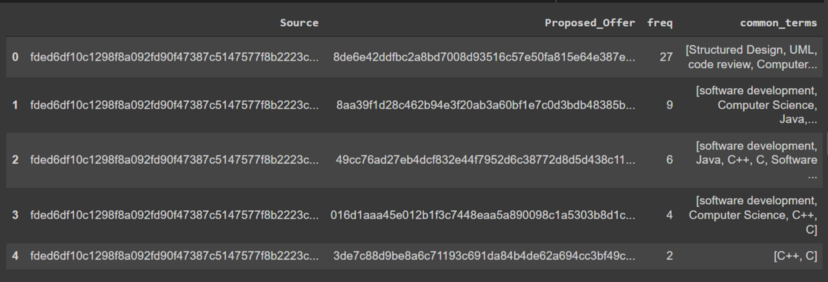
\includegraphics[width=\linewidth,keepaspectratio]{kg17}
			\end{center}	
			
			{\tiny (Ref: How to Build a Knowledge Graph with Neo4J and Transformers - Walid Amamou)}	
			
\end{frame}

%%%%%%%%%%%%%%%%%%%%%%%%%%%%%%%%%%%%%%%%%%%%%%%%%%%%%%%%%%%
\begin{frame}[fragile]\frametitle{Results}

In graph visual:

			\begin{center}
			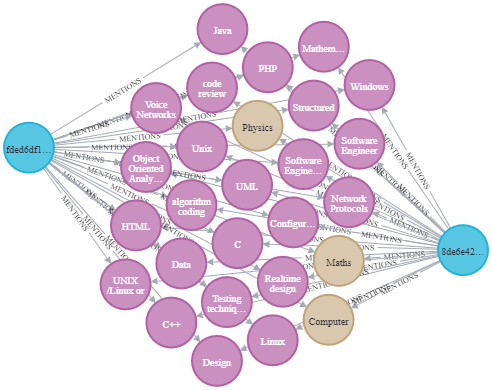
\includegraphics[width=0.6\linewidth,keepaspectratio]{kg18}
			\end{center}	
			
			{\tiny (Ref: How to Build a Knowledge Graph with Neo4J and Transformers - Walid Amamou)}	
			
\end{frame}

%%%%%%%%%%%%%%%%%%%%%%%%%%%%%%%%%%%%%%%%%%%%%%%%%%%%%%%%%%%
\begin{frame}[fragile]\frametitle{Run Queries}

To find out the most in demand skills:

\begin{columns}
    \begin{column}[T]{0.6\linewidth}
		
			\begin{lstlisting}
			query = """
			MATCH (s:SKILLS)<-[:MENTIONS]-(o:Offer)
			RETURN s.name as skill, count(o) as freq
			ORDER BY freq DESC
			LIMIT 10
			"""
			res = neo4j_query(query)
			res
			\end{lstlisting}
    \end{column}
    \begin{column}[T]{0.4\linewidth}
			\begin{center}
			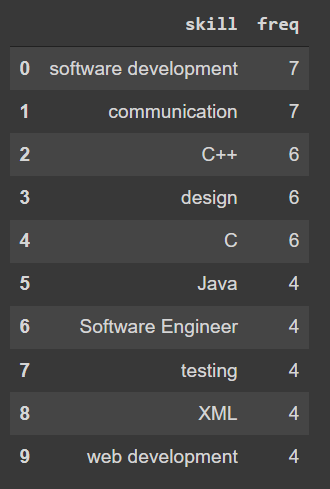
\includegraphics[width=0.8\linewidth,keepaspectratio]{kg19}
			\end{center}	
			
			{\tiny (Ref: How to Build a Knowledge Graph with Neo4J and Transformers - Walid Amamou)}	
    \end{column}			
\end{columns}
			
\end{frame}

%%%%%%%%%%%%%%%%%%%%%%%%%%%%%%%%%%%%%%%%%%%%%%%%%%%%%%%%%%%
\begin{frame}[fragile]\frametitle{Run Queries}

To find skills that require that highest years of experience:

\begin{columns}
    \begin{column}[T]{0.6\linewidth}
		
			\begin{lstlisting}
query = """
MATCH (s:SKILLS)--(r:Relation)--(e:EXPERIENCE) where r.type = "EXPERIENCE_IN"
return s.name as skill,e.years as years
ORDER BY years DESC
LIMIT 10
"""
res = neo4j_query(query)
res
			\end{lstlisting}
    \end{column}
    \begin{column}[T]{0.4\linewidth}
			\begin{center}
			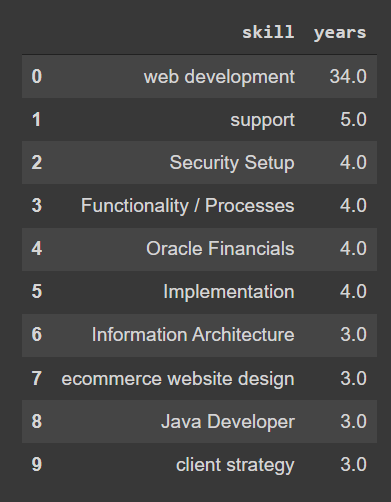
\includegraphics[width=\linewidth,keepaspectratio]{kg20}
			\end{center}	
			
			{\tiny (Ref: How to Build a Knowledge Graph with Neo4J and Transformers - Walid Amamou)}	
    \end{column}			
\end{columns}
			
\end{frame}

%%%%%%%%%%%%%%%%%%%%%%%%%%%%%%%%%%%%%%%%%%%%%%%%%%%%%%%%%%%
\begin{frame}[fragile]\frametitle{Run Queries}

To find  pair of skills co-occur the most:

\begin{columns}
    \begin{column}[T]{0.6\linewidth}
		
			\begin{lstlisting}
neo4j_query("""
MATCH (s1:SKILLS)<-[:MENTIONS]-(:Offer)-[:MENTIONS]->(s2:SKILLS)
WHERE id(s1) < id(s2)
RETURN s1.name as skill1, s2.name as skill2, count(*) as cooccurrence
ORDER BY cooccurrence
DESC LIMIT 5
""")
			\end{lstlisting}
    \end{column}
    \begin{column}[T]{0.4\linewidth}
			\begin{center}
			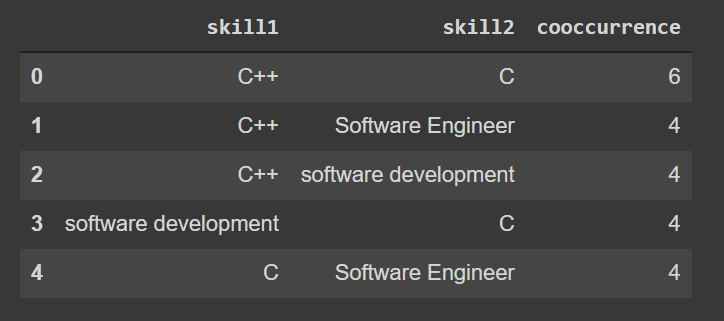
\includegraphics[width=\linewidth,keepaspectratio]{kg21}
			\end{center}	
			
			{\tiny (Ref: How to Build a Knowledge Graph with Neo4J and Transformers - Walid Amamou)}	
    \end{column}			
\end{columns}
			
\end{frame}

%%%%%%%%%%%%%%%%%%%%%%%%%%%%%%%%%%%%%%%%%%%%%%%%%%%%%%%%%%%
\begin{frame}[fragile]\frametitle{Conclusion}

\begin{itemize}
\item How to leverage transformers based NER and spacy’s relation extraction models to create knowledge graph with Neo4j.
\item In addition to information extraction, the graph topology can be used as an input to another machine learning model. 
\end{itemize}
	  
\end{frame}






%%%%%%%%%%%%%%%%%%%%%%%%%%%%%%%%%%%%%%%%%%%%%%%%%%%%%%%%%%%
\begin{frame}[fragile]\frametitle{References}

\begin{itemize}
\item DAT278x - From Graph and Knowledge Graph - EdX course
\item A Universe of Knowledge Graphs -  Dr. Maya Natarajan, Dr. Jesus Barrasa
\item How to Build a Knowledge Graph with Neo4J and Transformers - Walid Amamou
\end{itemize}
	  
\end{frame}


% %%%%%%%%%%%%%%%%%%%%%%%%%%%%%%%%%%%%%%%%%%%%%%%%%%%%%%%%%%%
% \begin{frame}[fragile]\frametitle{Sample Picture Inclusion}

% \begin{center}
% \includegraphics[width=0.8\linewidth,keepaspectratio]{myphoto}
% \end{center}	  
% \end{frame}

% %%%%%%%%%%%%%%%%%%%%%%%%%%%%%%%%%%%%%%%%%%%%%%%%%%%
% \begin{frame}[fragile] \frametitle{Sample Code Listing}
% \begin{lstlisting}
% import aaa
% \end{lstlisting}

% \end{frame}

% %%%%%%%%%%%%%%%%%%%%%%%%%%%%%%%%%%%%%%%%%%%%%%%%%%%%%%%%%%%
% \begin{frame}[fragile]\frametitle{Sample Two Columns Slide}
% \begin{columns}
    % \begin{column}[T]{0.6\linewidth}
      % \begin{itemize}
		% \item aaa
	  % \end{itemize}

    % \end{column}
    % \begin{column}[T]{0.4\linewidth}
      % \begin{itemize}
		% \item bbb
	  % \end{itemize}
    % \end{column}
  % \end{columns}
% \end{frame}

% %%%%%%%%%%%%%%%%%%%%%%%%%%%%%%%%%%%%%%%%%%%%%%%%%%%%%%%%%%%%%%%%%%%%%%%%%%%%%%%%%%%
% \begin{frame}[fragile]\frametitle{Sample Tabular Data}

% aaa

% \begin{tabular}{|c|c|}
	% \hline
	% Platform & Time (s) \\
	% \hline \hline
	% Python & $\sim$1500.0 \\
	% \hline
	% NumPy & 29.3 \\
	% \hline
	% Matlab & $\sim$29.0 \\
	% \hline
	% Octave & $\sim$60.0 \\
	% \hline
	% Blitz (C++) & 9.5 \\
	% \hline
	% Fortran & 2.5 \\
	% \hline
	% C & 2.2 \\
	% \hline
% \end{tabular}

% \end{frame}
